%%
%% Copyright Guy Taylor 2012
%%
%%

%% config the formatting
\documentclass[bsc,logo,plainprepages,parskip,abbrevs,10pt]{infthesis}

%% define the type of doc
\course{Software Engineering}
\project{Fourth Year Project Report}

%% import extra packages needed
%\usepackage{natbib}
\usepackage{url}
\usepackage{listings}
\usepackage{acronym}
\usepackage{graphicx}
\usepackage{wrapfig}

%% information about the doc
\title{Design and Implemenation of a Low Power Wireless Medical Respirotory Network}
\author{Guy Taylor}
\submityear{2012}
\graduationdate{June 2012}

%% abstract
\abstract{
The Respire device provides wireless low-power, unobtrusive respiratory monitoring of patients by use of
accelerometers to detect breathing movements. Implementation of a wireless networking capability
for this device will facilitate its widespread use in diagnosis and clinical management of respiratory
disease. The aim of this project was to develop Respire network firmware based on the \acf{TDMA}
method of network channel access, which was concluded to be the
only large-network (\textgreater 6 device constraint of the Respire hardware) method suitable for the Respire. I
produced and tested operational and debugging firmware for project development, which led to
identification of problems implementing \ac{TDMA} with the Send-Receive function of the low-power
nRF24l01+ radio onboard the Respire device. This has precluded testing of my design with the Respire
devices in a large-network environment. An important aspect of firmware development was to
include power-saving features where possible (\eg x\% reduction in power use when implementing
delays relative to code provided by the manufacturer). The project material (firmware, debugging
and testing systems) provides a basis for future development and application of the Respire family of
devices.
}

%% Now we start with the actual document.
\begin{document}

%% First, the preliminary pages
\begin{preliminary}

%% This creates the title page
\maketitle

%% Acknowledgements
\begin{acknowledgements}
  Todo
\end{acknowledgements}

%% Next we need to have the declaration.
\standarddeclaration

%% Create the table of contents
\tableofcontents

%% If you want a list of figures or tables, uncomment the appropriate line(s)
\listoffigures
\listoftables

\begin{acronym}
\acro{TDMA}[TDMA]{Time Division Multiple Access}
\acro{FDMA}[FDMA]{Frequency-Division Multiple Access}
\acro{CSMA}[CSMA]{Carrier Sense Multiple Access}
\acro{ECG}[ECG]{Electrocardiogram}
\acro{RISC}[RISC]{Reduced Instruction Set Computer}
\acro{MCU}[MCU]{Microcontroller}
\acro{PRS}[PRS]{Peripheral Reflex System}
\acro{DMA}[DMA]{Direct Memory Access}
\acro{SWD}[SWD]{Serial Wire Debugging}
\acro{SWO}[SWO]{Serial Wire Out/Viewer}
\acro{I/O}[I/O]{Input/Output}
\acro{RTC}[RTC]{Real Time Clock}
\acro{USART}[USART]{Universal asynchronous receiver/transmitter}
\acro{CMU}[CMU]{Clock Managment Unit}
\acro{EMU}[EMU]{Energy Managment Unit}
\acro{PHY}[PHY]{Physical}
\acro{DL}[DL]{Data Link}
\acro{GPIO}[GPIO]{General Purpose Input Output}
\acro{FIFO}[FIFO]{First In First Out}
\acro{OS}[OS]{Operating System}
\acro{API}[API]{Application Programming Interface}
\acro{SPI}[SPI]{Serial Peripheral Interface (Bus)}
\acro{NRF24}[NRF24]{Nordic nRF24L01+ Radio}
\acro{PCB}[PCB]{Printed Circuit Board}
\acro{ISM}[ISM]{Industrial, Scientific and Medical}
\end{acronym}

\end{preliminary}

%%%%%%%%
%% Include your chapter files here. See the sample chapter file for the basic
%% format.

%%
%% Copyright Guy Taylor 2012
%%
%%

\chapter{Introduction}

\section{Introduction}

The concept of medical equipment that enables unobtrusive wireless monitoring of various human
life-signs has been a recurring theme in science fiction for years\cite{StarTrekStarFleetTechnicalManual1986}, but only recently have
technological advancements been made that might help realize these possibilities and bring them to
market. Realizing the dream of detecting medical conditions early, even before they produce readily-detectable
symptoms, in people fit or ill entails both continuous monitoring of all vital signs (such as
pulse, respiratory rate and temperature) and their analysis in relation to known conditions or
detection trends over the person’s life. This possibility has sparked initiatives such as a 10 million
dollar prize for a "Tricorder"\cite{XprizeHealth2012} and new research into ways of measuring and analysing vital
signs.


In order for the researchers and medical staff to fully achieve these aims, hardware designers and
programmers need to produce platforms that are unobtrusive, easy-to-use and of low cost. A new
generation of devices and technologies are being designed and perfected as part of the research
process to system development, incorporating features such as the latest generation of low-power
\ac{MCU} and wireless transceivers suitable both for patient-monitoring devices
and, in a broader context, for small  consumer-electronics fitness aids\cite{Jawbone2012, Fitbit2012}.

\begin{wrapfigure}{r}{0.5\textwidth}
  \vspace{-10pt}
  \begin{center}
    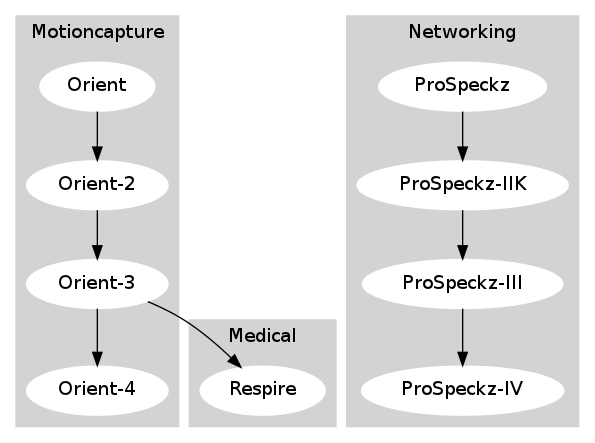
\includegraphics[width=0.4\textwidth, keepaspectratio=true]{images/respire_family_history.png}
  \end{center}
  \caption{Respire family history}
  \vspace{-10pt}
\end{wrapfigure}

The Centre for Speckled Computing within the School of Informatics, University of
Edinburgh, has produced several generations of small low-power sensor platforms for use
in motion capture and general research. These Orient\cite{Orient2012} and ProSpeckz\cite{ProSpeckz2012} devices
have facilitated hardware development and research, embracing the rapid prototype
design methodology. Building on the success of research projects with these devices, it
became apparent that more specific versions were needed both to enable new research and to
reduce the limitations of such a generic platform. This requirement, linked to the rapid development
of suitable microelectronics, has led to the production of two new devices built in tandem. These are
(1)The Respire, a respiratory monitoring device inspired by the Orient-3 motion-capture platform
but built from the ground up for low-power in a smaller, lighter package and (2) the new Orient-5,
upgrading the Orient motion-capture series to the latest generation of technology.

\section{Respiratory Monitoring}

\begin{wrapfigure}{r}{0.3\textwidth}
  \vspace{-10pt}
  \begin{center}
    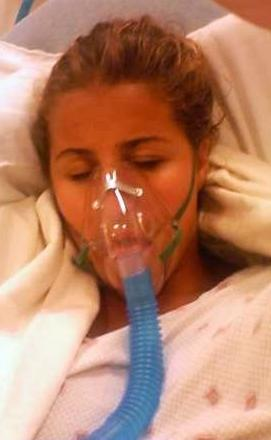
\includegraphics[width=0.2\textwidth, keepaspectratio=true]{images/Plastic_oxygen_mask_on_an_ER_patient.jpg}
  \end{center}
  \caption[Face Mask]{Face mask \cite{FaceMaskImg}}
  \vspace{-10pt}
\end{wrapfigure}

\subsection{Measurement of Respiratory Airflow}
At present the most effective and widely used systems for continuous respiratory monitoring in
people require the patient (or interested subjects) to wear a nasal cannula or face mask and directly
measure respiratory airflow. However, when not necessary for the medical administration of gasses,
these systems are both invasive and uncomfortable for the patient\cite{NasalCannula2011}. Whilst accurate, they
restrict patient movement and are unlikely to be used for long periods of time for monitoring alone.
It has however been demonstrated that an adaptation of the Respire accelerometer-based device
fitted to a nasal cannula could produce a workable wireless monitoring system.

\begin{wrapfigure}{l}{0.3\textwidth}
  \vspace{-10pt}
  \begin{center}
    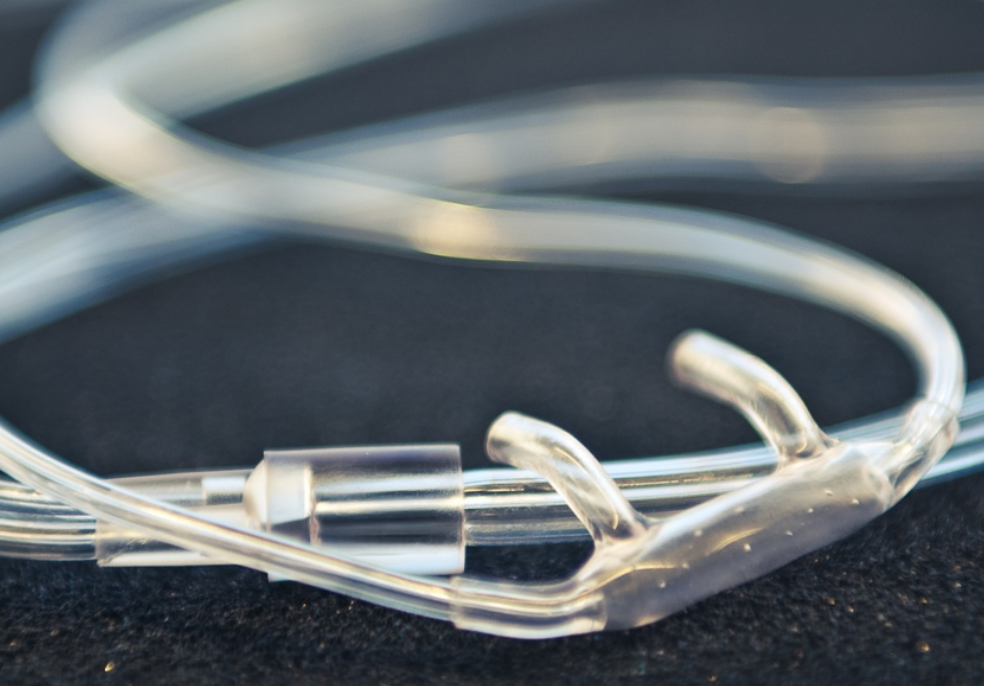
\includegraphics[width=0.2\textwidth, keepaspectratio=true]{images/nasal_canula.png}
  \end{center}
  \caption[Face Mask]{Nasal cannula \cite{SpecknetFlyer}}
  \vspace{-10pt}
\end{wrapfigure}

\subsubsection{Diaphragm Rotation}
The correlation between the rotation of the diaphragm (as measured by acceleration) and the
respiratory rate was recently shown to be accurate enough for medical use by the University of
Edinburgh team who designed the Respire device \cite{BatesLingMannArvind2010}. This non-invasive
means to measure the respiratory rate is achieved by affixing a small accelerometer onto
the patient's lower chest.


\subsubsection{\acf{ECG}}
It is also been shown that single or multiple lead \ac{ECG} can give a reasonable indication of respiratory
frequency ($\pm4$ breaths a minute) and is more independent of the wearer's movements than
accelerometers \cite{ZhaoZhaoQun2008, BoyleBidargaddiSarelaKarunanithi2009}.

\subsection{Usages}
Currently the main use of continuous respiratory monitoring is in intensive
care wards. In respiratory wards there is mainly only the use of non-continuous
60-second breath count measurements with the noting of breathing depth only in vague
terms \cite{Hunter2008}. It however is an increasing field of study, as with the availability of continuous measuring
devices, new diagnostics can be found. This mirrors the previous evolution of other medical
monitoring devices such as heart rate monitors and blood glucose analyzers.
% TODO (COPD ?) %
An example of the potential diagnostic power and applications of continuous respiratory
monitoring is in Sleep Apnoea. With real-time data collection, professionals can quickly diagnose the
condition whilst the patients can be alerted of their onset, thus preventing harm by waking up (ref). % TODO
For this to be successful the system must be unobtrusive enough to
sleep with and be reliable enough to be life-critical.
The overall goal of this project is to support the role of the medical
professionals and research staff in their attempts to find more
effective, comfortable and cheaper ways to diagnose and manage
respiratory conditions. To this end, the devices and designs are there specifically to enable this
purpose and not to break ground in other areas.
To enable collection of continuous respiratory rates, a device that can record and transmit
respiratory data wirelessly whilst still being small and light enough to be carried by the patient is
required. The device should be unobtrusive and simple to use, whilst decreasing the complexity of
the current system. This device should be suitable for use in hospitals at the required technical and
hygiene standards, in an environment that may contain multiple Respire devices and other
electronically controlled systems

\section{Goal}
This project proposes one solution for a new low power radio interface for the Respire device to
facilitate the more general use in a clinical setting.



%%
%% Copyright Guy Taylor 2012
%%
%%
\chapter{Background}

\section{Background}
Initial trials at the University of Edinburgh established that breathing movements and respiratory
frequencies could be measured accurately and reproducibly using accelerometers attached to the
chest of human subjects (including hospital patients), reaching levels of 96\% accuracy\citer{BatesLingMannArvind2010}.
It was therefore decided to produce a custom piece of hardware dedicated
to this task that might be suitable for longer-term clinical use. The accelerometer device used in the
trial was a prototype based on the Orient-3 wireless sensor platform originally designed for use in
real-time motion capture. For the trial however, the monitoring system did not use the wireless
transceiver but instead used off-line analysis.

\begin{wrapfigure}{r}{0.45\textwidth}
  \vspace{-10pt}
  \begin{center}
    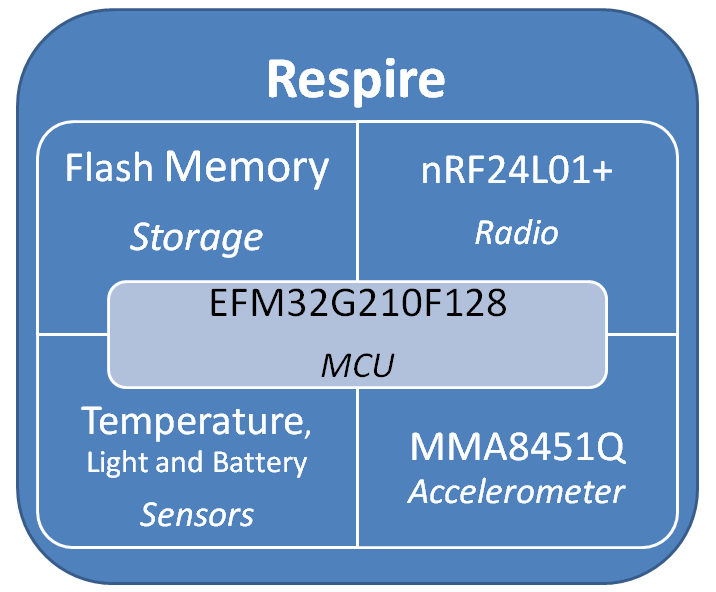
\includegraphics[width=0.35\textwidth, keepaspectratio=true]{images/respire_block.png}
  \end{center}
  \caption[Respire Block Diagram]{Respire block diagram}
  \vspace{-10pt}
\end{wrapfigure}

With the aim to reach medical trials, a smaller and lower-powered device was designed to allow
longer-term monitoring for further investigations of accelerometer-based respiratory monitoring on
patients The new hardware was named the Respire and is a significant improvement over the
prototype device. The Respire integrates four key components of the prototyped Orient-2/3 onto a
single more accessible device to allow further development and testing: a \ac{MCU},
accelerometer, radio and flash memory. However, the original Orient-3 firmware was incompatible
with the Respire and therefore a new firmware needed to be designed and implemented, with an
emphasis on reducing the power requirements of the system.

\section{Power Management}
To calculate the power needed to run a device you first need to measure the power use during
active use \(P_{active}\), power use during sleeping \(P_{sleep}\) and the percentage of time in a state of
activity \(Duty\).
\[
  P_{average} = D x P_{active} + (1-D) x P_{sleep}
\]
\[
  P_{active} \gg P_{sleep}
\]
It is most common however that \(P_{active}\) and \(P_{sleep}\) are fixed or only small reductions can be
made. It is therefore most effective in normal applications to reduce the duty, this reduction is most
assisted by faster wake up periods\citer{Edgar2003}.


\begin{wrapfigure}{l}{0.5\textwidth}
  \vspace{-10pt}
  \begin{center}
    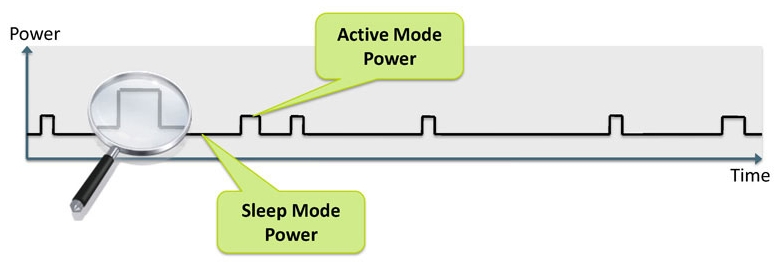
\includegraphics[width=0.4\textwidth, keepaspectratio=true]{images/lowenergysystemsoverview_croped.jpg}
  \end{center}
  \caption[Duty Graph]{Duty graph\citer{EFM32Tech}}
  \vspace{-10pt}
\end{wrapfigure}

In any small wireless devices the main power consumer is the radio during use, therefore it is key to
minimise its duty cycle. Mediation devices exist between the edge nodes and the core of a network,
allowing data to be buffered and processed away from the edge. This mediation allows the edge
devices to ``sleep'' more predictably and with greater duration and depth, decreasing the edge
power needs\citer{Edgar2003}.


This system of moving the power towards the centre of the network is more effective in hierarchical networks
where there is a clear distinction, \eg by a larger battery, between the nodes
and the mediation devices. This allows the mediation device to be awake for
longer without the battery expectancy of the global networks decreasing.

\section{Respire Device Components}

\subsection{Energy Micro EFM32 \ac{MCU}}

\begin{wrapfigure}{r}{0.8\textwidth}
  \vspace{-10pt}
  \begin{center}
    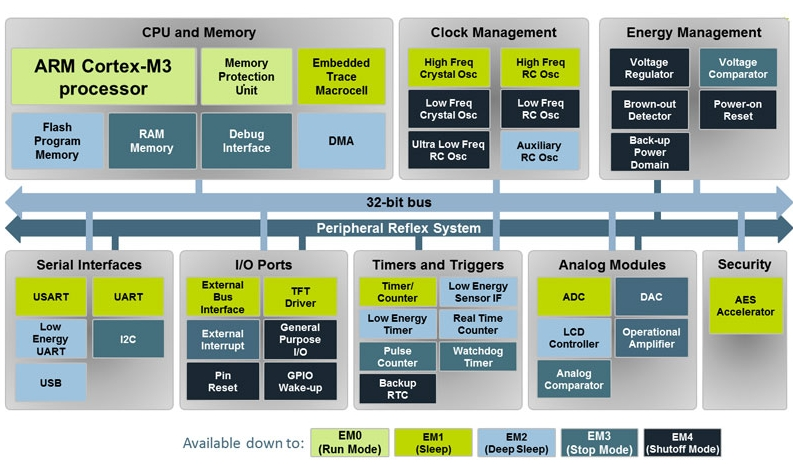
\includegraphics[width=0.7\textwidth, keepaspectratio=true]{images/efm32_block_croped.jpg}
  \end{center}
  \caption[EFM32 Block Diagram]{EFM32 block diagram\citer{EFM32Tech}}
  \vspace{-10pt}
\end{wrapfigure}

The Energy Micro EFM32 series of \ac{MCU} is a system-on-a-chip designed from the bottom
up for low energy applications. At the core of the EFM32 is an ARM Cortex-M3 \ac{MCU} enabling the
power and flexibility to reduce energy needs by decreasing duty time and closely interacting with its
peripherals. In the same silicon to the \ac{MCU} is an array of specially designed low-power modules,
many of them, that are independently wired together allowing \ac{MCU} free communication and
interaction enhanced by a \ac{DMA} controller.

\subsection{ARM Cortex-M3}
The ARM Cortex-M3 is a 32-bit Harvard style, \ac{RISC} \ac{MCU}. It is designed
around the ARMv7 instruction set with the addition of Thumb
and Thumb-2 compressed instruction sets. The Cortex-M is the sub series dedicated to low power
system-on-a-chip \acp{MCU}, with the Cortex-M3 being specifically for realtime applications.


The Cortex-M3 series was designed to both provide good performance with low power but also
decrease the complexity of programming, the normally complex 8 and 16-bit architectures. This
reduction in complexity is mainly achieved by the use of assembly free interrupts and the full
standardisation of configurations through the use of memory mapped registers. This standardisation
allows the many implementations of Cortex-M3, with different system-on-a-chip peripherals, to be
easily learnt. The assembly free interrupts allow all code to be viewed in a single language and thus
preventing hidden or obscured processes. This ease of implementation is assisted by a full debugging
subsystem, with optional in-circuit emulator, accessible via a new 2 to 3 pin interface reducing the
size on the device and thus allowing debugging be kept in the production layout. This new debugging
interface, \ac{SWD}, has a built in ability to directly communicate back to the
debugger using the optimal 3rd, \ac{SWO}, pin. With the \ac{SWO} the programmer can use
standard consoles printing techniques without disruption of the program flow.\citer{EnergyMicro2011}


The Thumb reduced instruction set is a 16-bit wide subset of the main ARM set that allows multiple
instructions to be compressed into a single instruction read, thus reducing \ac{IO} latency. The Thumb-2
instruction set extend thumb set by the utilising 32-bit instructions and thus provide more
functionality and packing, thus providing a 30\% improvement. This combination lowers the speed to
power ratio and also the program memory needed. This performance is also achieved with the
simple, false always, branch speculation within the three stage pipeline.\citer{Arm2012}


The Cortex-M3's most important improvements are the new interrupt system and single bit
manipulation system. The new interrupt system reduces interrupt latency, allows direct wake from
sleep and also allows chaining, with priority. chaining of interrupts significantly reducing interrupt
latency in instances where interrupts are likely to happen simultaneously. The priority system allows
key events to be reordered reducing the chance of delay, producing a more deterministic system. A
new bit manipulation system allows individual bits to be changed without reading, modifying and
writing the whole byte, reducing \ac{IO}. The ``bit-banding'' is also combined with the previous
generation unaligned memory system allowing single bit, byte, half word and the full 32-bit word to
be uniquely addressed.\citer{EnergyMicro2011}

% TODO
% Throughout all ARM architecture there is the CIMIS standardisation.....

\subsection{\acf{PRS}}

\begin{wrapfigure}{l}{0.5\textwidth}
  \vspace{-10pt}
  \begin{center}
    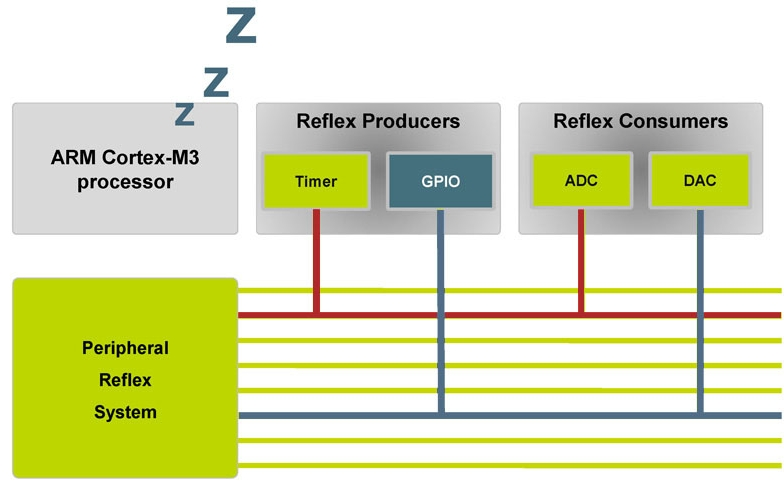
\includegraphics[width=0.4\textwidth, keepaspectratio=true]{images/peripheralreflexsystem_croped.jpg}
  \end{center}
  \caption[EFM32 \ac{PRS} Diagram]{EFM32 \ac{PRS} diagram\citer{EFM32Tech}}
  \vspace{-10pt}
\end{wrapfigure}

The \ac{PRS} is a technology that allows the peripherals in the system-on-a-
chip, external to the \ac{MCU}, to independently interact and thus not force the \ac{MCU} to wake from
sleep. To enable such control, the system has predefined production and consumption interfaces on
each module, these range from automated \ac{ADC} every second triggered by the \ac{RTC} to using receipt
of \ac{USART} data to trigger switching of a device pin. Many of these peripherals clock independently of
the \ac{MCU} so this system can even work in the deepest sleep states.

\subsection{\acf{CMU} and \acf{EMU}}

\begin{wrapfigure}{r}{0.4\textwidth}
  \vspace{-10pt}
  \begin{center}
    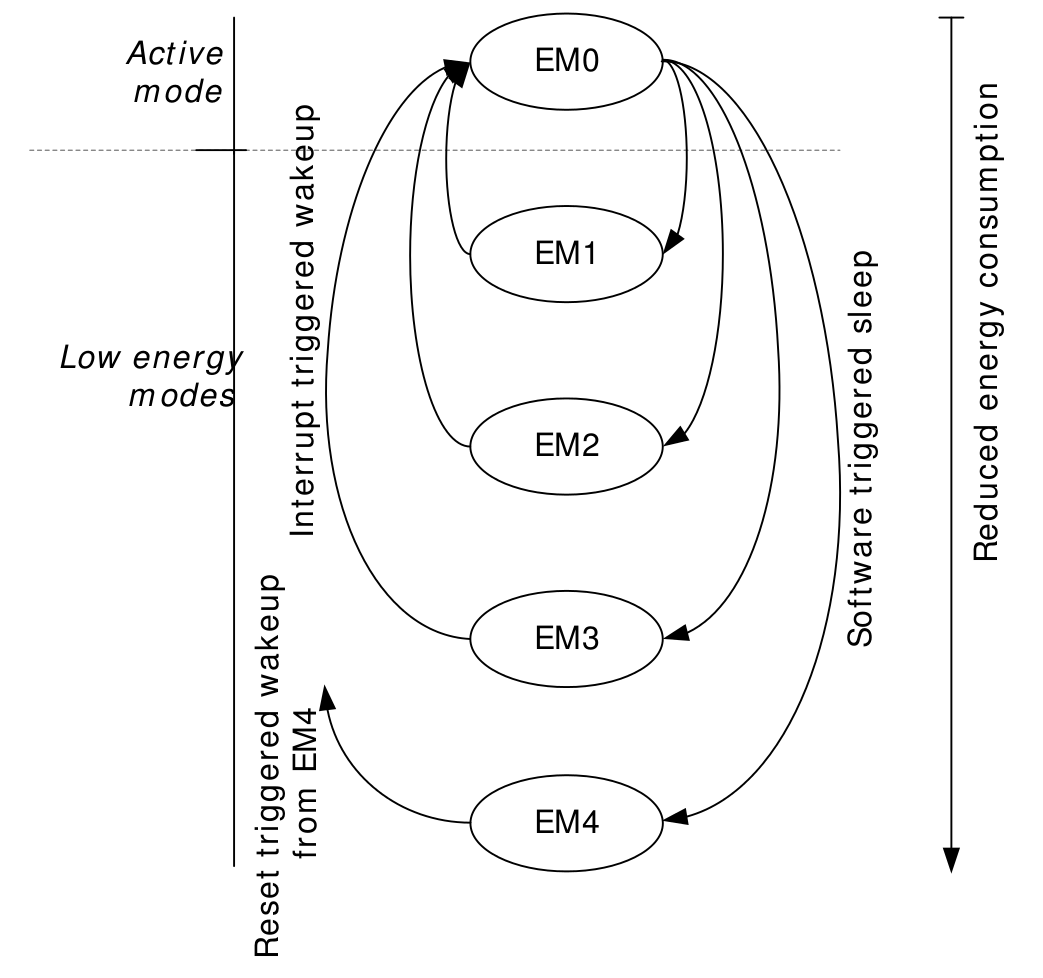
\includegraphics[width=0.3\textwidth, keepaspectratio=true]{images/efm32_sleep_states.png}
  \end{center}
  \caption[EFM32 \ac{EMU} Diagram]{EFM32 \ac{EMU} diagram\citer{EFM32Ref}}
  \vspace{-10pt}
\end{wrapfigure}

The EFM32s ground up approach of designing all models in the system, except from the \ac{MCU} and \ac{DMA} controller,
allows a powerful clock and energy management system that allows individual clocking and enabling
of each subsystem allowing modules to consume no power when not in use. The clock management
system also enables several clock to be chosen for each module, allowing the programmer is most
effectively choose the set of clocks needed. Thank you management system also extend directly into
the \ac{MCU}, allowing extra sleep states to be added to the Cortex-M3. These extra sleep states allow
the \ac{MCU} to gradually decrease the number of high frequency clocks the maintain state and
also includes full hibernation of the chip with only the externally clocked subsystems
enabled. From these sleep states EFM32 has a fast wake-up time allowing shorter burst
periods and deeper sleeps.

\subsection{Nordic nRF24L01+}
The Nordic nRF24L01+ (hereafter referred to as NRF24) is a low-power digital radio
designed to work in the 2.4Ghz ISM radio bands. The radio enables fast 2Mbit transfer
between devices but only supports half duplex communications and therefore cannot transmit and
receive data simultaneously.

\subsection{MMA8451Q Accelerometer}
This component was included to support the high-accuracy measurements needed to monitor
breathing movements in a small, low-energy package.

\subsection{Flash Memory}
A 64-Mbit flash memory chip is included in the Respire to facilitate offline storage of sensor data
when no network is available.



%%
%% Copyright Guy Taylor 2012
%%
%%

\chapter{Design}

\section{The Goal}
My task was to design and implement a low power wireless network for the Respire devices. This
network should be effective in both reducing the power consumption of the Respire device and
allow the required data to be accessible in real-time. An extension of the design should allow bulk
data upload if the device re-enters the network after a period of disconnection. The network should
also allow a simple device initialisation within the network, so as to be as "plug-and-play" as possible
and also allow the device to actively maintain a connection as the patient moves between relays or
networks. The network should allow relay devices to extend the signal from the data collection
destination, so simplifying any wiring requirements.

\section{Requirements}
The Respire is intended to be used initially in a hospital environment but with the hope to later
extend it for use in a patient’s residence. There is therefore a requirement for it to be legal for public
use with no assumption of consistent infrastructure. Within hospitals it is required not to interact
with other equipment or prevent use of required services.


The Respire should be as simple as possible as the user at home is not expected to be
knowledgeable in the area and the medical professional should not be burdened with configuration
or maintenance. This also reduces both cost and chance of failure, enabling access to more patients
and reducing patients risk during failures.


The Respire network should allow the patient greater freedom to move around a room or building
without the need to be tethered to sensor, power or communications equipment. This should help
promote mobility and, in consequence, aid recovery and reduce hospital stay.
The Respire should be able to produce real-time data when needed but also be able to store and
then later transmit the data when connections permit. A fully functioning Respire network needs to
be capable of transmitting 3x14-bit samples at sample rate of 12.5Hz for effective respiratory
monitoring (Mann, J; personal communication).


\section{The Device}
The Respire consists of a single self contained \ac{PCB} with attached battery. The PCB contains the
central microcontroller, low power radio with antenna, three-axis accelerometer and flash storage.
At every level the Respire tries to reduce the power needs (\eg by reducing the chip count), and thus
each device selected is designed to be used in low power environments. Attributes of the Respire
include:-\\
\large{Strengths}
\begin{itemize}
  \item A single 32bit ARM Cortex-M3 microcontroller, enabling local data processing.
  \item All low power chips by design.
  \item Devices have low power sleep states, including four in the microcontroller.
  \item The radio transmits with a high bandwidth, allowing shortened duty cycles.
\end{itemize}
\large{Weaknesses}
\begin{itemize}
  \item Proprietary radio \ac{PHY}/\ac{DL} layer, non-standard and sufficiently different to prevent implementation of a standard.
  \item Problematic state machines due to sleep states.
\end{itemize}

\section{Network Design}
\begin{wrapfigure}{r}{0.7\textwidth}
  \vspace{-10pt}
  \begin{center}
    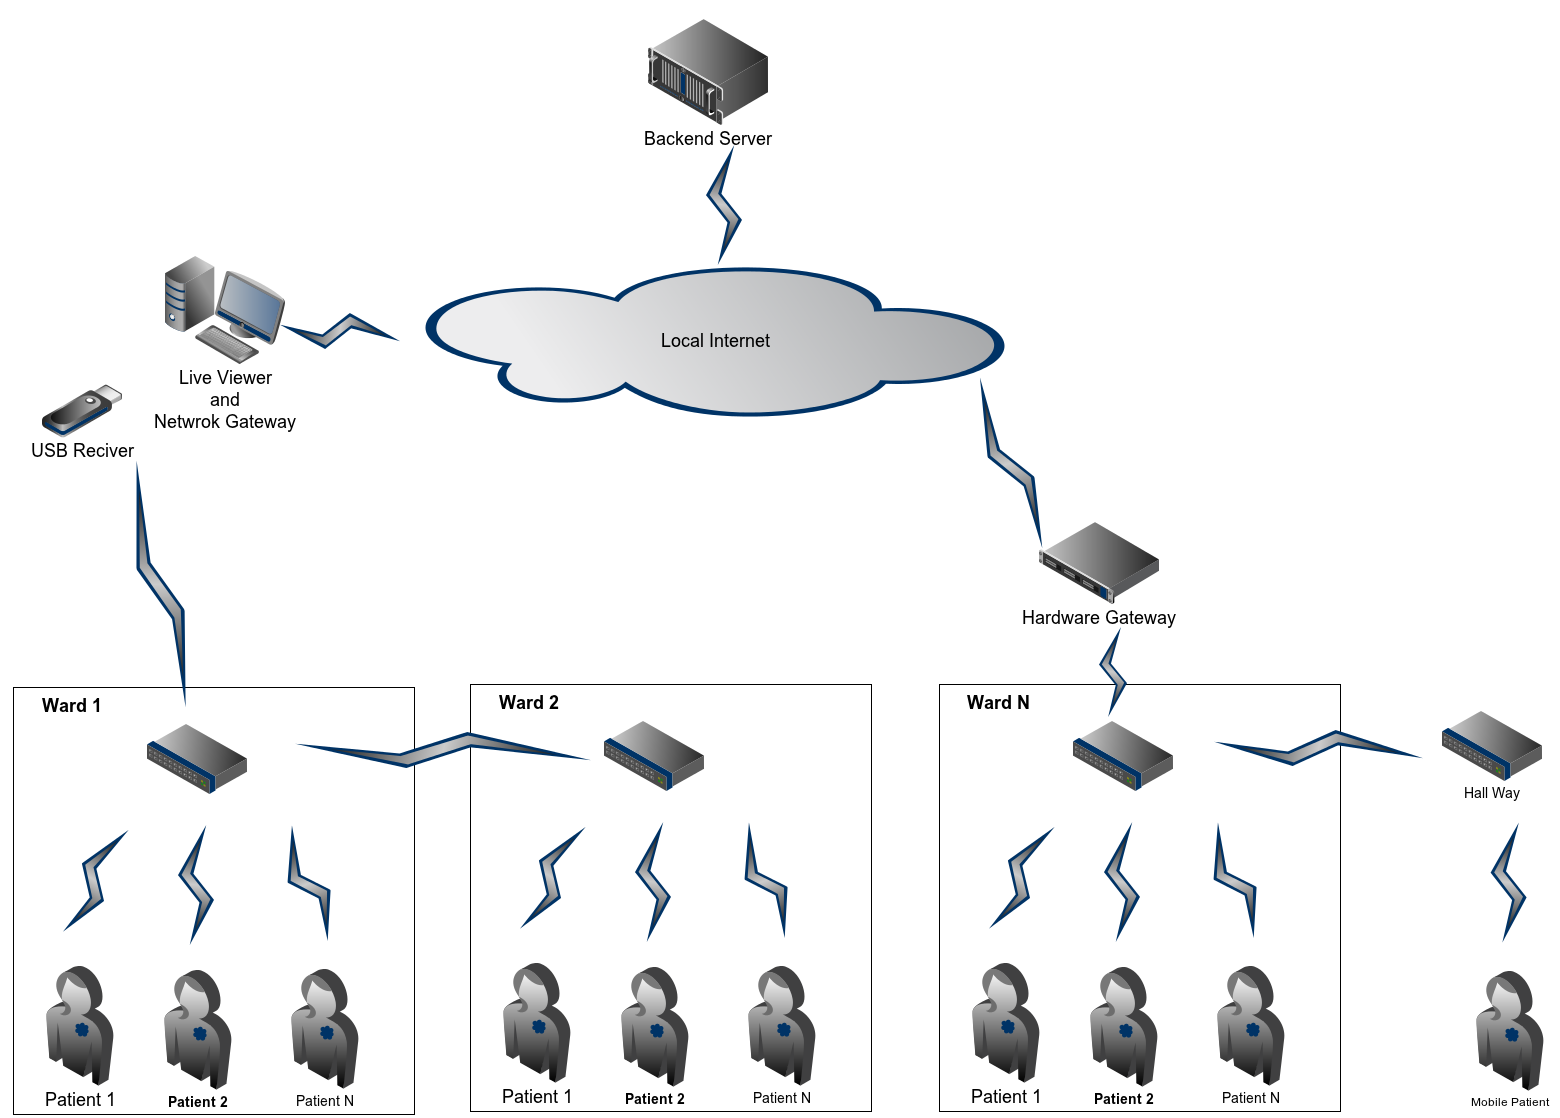
\includegraphics[width=0.6\textwidth, keepaspectratio=true]{images/respire_network.png}
  \end{center}
  \caption{Network Design}
  \vspace{-10pt}
\end{wrapfigure}
In this project I will propose a design for a low power wireless network system, this will be laid out in
a layered approach. Due to the unique hardware of the Respire no previous network has been
produced at the time of commencing this project address an entire radio stack by designing the
separate layers up the design will try and separate out the separate components creating a layered
and modular approach.

\subsection{Multiplexing}
As many Respire devices will be working in the same area there is a requirement that some sort of
multiple access system is implemented. In the wireless, and wired, domain there are three main
groups of multiplexing; \ac{TDMA}, \ac{FDMA} and \ac{CSMA}.

\subsubsection{\acf{FDMA}}
FDMA separates the signal spectrum into several channels, each with its own unique frequency
range. Each separate device then only transmits in its allotted channel. This provides the maximum
single throughput per device but comes with the requirement of either a separate receiver per
frequency or a more-expensive and energy-intensive broad frequency receiver. \ac{FDMA} is typically
used in managed environments, where one can guarantee each device has its own frequency.
\ac{FDMA} cannot be effectively implemented on the \ac{NRF24} as it cannot receive on more than one
channel and channel-hopping would be less effective than \ac{TDMA}. This would however reduce the
risk of noise on a single channel that \ac{TDMA} is susceptible to.

\subsubsection{\acf{CSMA}}
\ac{CSMA} has several variations all based around a single concept; that is, a device that wishes to
transmit, first senses the spectrum to ascertain whether it is free to transmit and if so, transmits its
data. The different variations diverge in respect to how they handle the situation if another device is
transmitting or the situation where more than one device has transmitted at the same time.
A key issue with \ac{CSMA} is the "hidden terminal problem", where two devices out of range of each
other but visible to a third compete for spectrum. One of the possible mitigation schemes is to use a
mediation device to share node information more globally in the network without high memory
costs, this could be achieved.


\ac{CSMA} however is not possible on the \ac{NRF24} as it does not adequately provide this built-in
ability or an effective equivalent software alternative to sense the channel. This would reduce the
need for accurate clocks and a highly managed \ac{TDMA} solution.


\subsubsection{\acf{TDMA}}
\ac{TDMA} allocates a time slot for each device, or as requested, for a single device to transmit within
uniquely. This distribution allows many devices to use a single channel without the need for sensing
or frequency change. However it requires an accurate time to be kept, and implemented on, for the
bandwidth to be used effectively. The requirement for accurate timekeeping and synchronisation
causes the greatest challenge for this type of multiplexing, because in modern electronics each
crystal (the component used to track time) has its own unique characteristics. The inability to keep
the clocks synchronised without adjustment can cause one device to transmit in another's time slot.
Time division multiplexing in its simplest form is most efficient when the data being transmitted is
both consistent and equally shared among the timeslots. This can be mitigated by giving devices that
need more bandwidth longer time periods but this requires predictable data requirements.
\ac{TDMA} also has an intrinsic but fixed maximum latency in communication and so can be used in time
critical applications, such as telecommunications. This benefit however, can only be achieved if each
device can be serviced in sufficient time before the cycle repeats. This often leads to \ac{TDMA} being
used in high frequency spectrum.


\ac{TDMA} was chosen for the Respire network as the radio can transmit at precise intervals and the
microcontroller provides an accurate clock. This choice had the benefit of allowing the network to
choose the least congested frequency band within the overcrowded \ac{ISM} bands and effectively
utilises Respires low power devices.

%TODO 
{discussion of why TDMA}


\subsection{Physical layer}
The \acf{PHY} layer of the \ac{NRF24} has many unique hardware features and to reduce power
it was decided to attempt to integrate these as much as possible.


The chip supports up to six separate receive pipelines each with its own address. This is designed to
support a small, many transmitters to single receiver, network (\eg Logitech’s Unifying brand of
wireless keyboards and mice). There are six separate receiving addresses but only two of these can 
be independently configured. This solution was therefore not used as the restriction of a network
size to six nodes per repeater was inadequate.

%TODO 
{add resspipline diagram}


An unusual feature of the chip is the use of the address as the sync in the air. This increases the
packet efficiency as it removes sections unused by the \ac{DL} layer and instead uses them instead. This
however restricts the address choices at the DL layer and disables any packet sniffing for debugging
or more custom \ac{DL} layer. As the address is sued as the sink pattern there is a need for many bit
changes within the sequence to give a high probability it is indeed the sync. This reduces the possible
addresses that can be used either by black listing the unacceptable addresses or by encoding them
and thus reducing the width (\eg Manchester encoding).


The Radio can only be in receive, transmit or sleep states so during the transition into and out of
transition or sleep to receiving, packets are lost. This will force any protocol to make sure that there
is sufficient time given pre and post transition to accommodate this limitation. This also forces the
device to needed to known ahead of time if it needs to transmit or receive a packet so it can
transition if needed to the correct state.


The silicon had a built in \ac{CRC} generator and checker enabling good packer corruption checking
during broadcast. The radio however does not attempt any forward correction and it was decided to
implement this in software as it is shown to have a low effectiveness\cite{NetworkDesign1998}.
The radio works within the 2.4GHz ISM band using a single or dual channel \ac{GFSK} modulated signal.
This provides 126 independent channels at 250kbps or 63 at 2Mbps and a speed-dependent
sensitivity rage of -94dBm to -82dBm. This use of the 2.4GHz ISM band provides worldwide licensing
for use at the power required and without the need to device identification. However due to the
relaxed licensing this region of the spectrum is highly noisy, with systems such as Bluetooth and
microwave ovens effectively denying service.

\subsection{\acf{DL} Layer}
Closely coupled to the multiplexing and \ac{PHY} properties of the radio, the \ac{DL} layer provides
a foundation that affects the direction of the layers above. The PHY layer has restricted the device
address to 2-5bytes, the one independent and 5 linked addresses and the packet size between 1-32bytes.


\subsubsection{Addressing}
Given the address limitations of the \ac{DL} layer, it was decided to only use two receiving addresses on
each device, one globally unique and one for broadcasts. This ability to broadcast and uniquely
address every device was chosen to both emulate the success of Ethernet and IEEE 802.15.4 but also
to simplify the higher link layer. This does require a globally unique address to be programmed
during production, however this can be readily automated and is not problematic. In development
the lower bytes of the microchips device ID were used, however if used in production this would
restrict the later choice of microcontroller and also not be perfectly unique as it is not the full ID. The
address width was chosen to be the maximum of 5 to both enhance the physical layer and expand
the total number of devices possible.

\subsubsection{Packet Assembly}
At this low level only a packet based design is possible with the radio. Enabling the built-in packet
assembly on the \ac{NRF24} was chosen to facilitate hardware \ac{CRC} checksums and reduce the
microcontroller duty cycle. The automated packet assembly will prepend a single "magic number"
byte along with the "to" address, length and a few command bits and then append a two byte CRC
checksum. This also was chosen to allow dynamic packet sizes at the \ac{DL} layer to again reduce power
at the radio by reducing broadcast time. The command bytes will not be used but cannot be
removed. The commands consist of bit fields indicating if the receiver should acknowledge the
packet and a short packet ID to assist in packet retransmission.

\subsubsection{\acf{SPI}}
The \ac{DL} layer is shared between the radio and microcontroller via a \ac{SPI} connection that is dedicated
to the radio. This therefore provides more than sufficient bandwidth for the application. The latency
is also low as there is no \ac{SPI} multiplexing and the radio provides an \ac{IRQ} signal to the \ac{MCU}.
A known silicon flaw in the EFM32G series does however increases the complexity of using the
double buffer, putting it beyond the scope of this project\cite{EnergyMicroErata2012}. The importance
of interrupts in \ac{TDMA} prevents the use of the popular FTDI \ac{MPSSE} series of chips due to the lack of
interrupt support.

\subsection{Network Layer}
The network layer abstracts the inner workings of the network to the application whilst also
monitoring and controlling the \ac{DL} layer. This is also the first layer solely within the \ac{MCU}
providing flexibility to the designer.
The network topology chosen for the project is a clustered-tree as this best encapsulates the
physical topology of a hospital; that is, many patients in many rooms with a few data collection
points. This topology also encapsulates the ideas of a Mediation Device with the differing power
availabilities (battery to larger battery or mains)\cite{4517407}.

\subsubsection{Connecting, Moving and Disconnecting to Networks}
There are two main categories of address registration in networks. The first actively requests
addresses from a central source using the DL layer broadcast (\eg \ac{DHCP}). The second listens to the
network and tries to attempt to join using the information learned (\eg \ac{NDP}). It was decided to
use a mixed model for the Respire network in an attempt to optimise the network.


Periodic broadcasts are sent with next available address to be used by a new child device. An
unconnected node listens for a broadcast, by first-found or strongest-signal, and then randomly
waits 1 to 16 more broadcasts from that relay, this prevent self denial of service on a full network
reset. After the wait the node will then transmit a connection request in the \ac{TDMA} block defined by
the address in the broadcast field (Add info on the event if the address is taken on attempted use
before first attempt). The relay will reply with accept or deny, with the denial reason. In failure, due
to packet collision by another device trying to connect, the 1 to 16 delay is repeated. If the denial
reason suggests an inability to connect to that relay, it should be blacklisted. This design allows
nodes to know if a network is accepting connections, the address to use and the additional
information in the broadcast (all before connecting) and also minimises denial of service and packet
collisions. Again this design allows effective device sleeping as during the wait periods there is a
known duration of sleep (Figure x). % TODO


On the device wishing to disconnect from the network, a simple disconnect request is sent. If the
relay does not receive an accept, it should still disconnect and assume the relay will remove it
through a timeout (Figure 2). This additional information sent to the parent allows fast reuse of the
time division slot in situations, such as busy hospital wards, where the parent is at capacity.
On the device wishing to transfer to a different relay in the same network, the device will first send a
disconnect request- with intent to transfer- to the current relay. Whether the last packet is received
or not, the device connects to the new relay. The last packet received from the previous relay
provides the ability, currently not used, for quick switching (Figure x). % TODO

\subsubsection{Addressing}
Along with a globally unique \ac{DL} Address the network layer will register for a transient network
address. This address has several purposes: it enables packet routing, is used as the \ac{TDMA} time slot
and controls the bandwidth allocation.


The address is a single byte divided into a upper and lower nibble. The upper nibble identifies the
connected relay and the lower identifies the node within the relay. This small address range was
chosen as after a network surpasses 256 nodes and relays it also surpasses the available bandwidth
for that channel. Several separate networks on independent channels would allow more than 255
devices.


The \ac{TDMA} time slot is decided by the device address. The initial period is separated into 128 relay
blocks which in turn are separated into 128 node blocks. This system guarantees that every device
connected to the network, even across relays, has a unique time slot to transmit in. The nodes’ radio
use is then condensed into a short period, allowing long periods of uninterrupted sleep, reducing
duty.


\subsubsection{\acf{DL} Layer Monitoring}
With more knowledge than the \ac{DL} layer, the network layer can make better decisions on power
management and buffer control than the \ac{DL} layer. It is also important for the network layer to be
aware of the \ac{DL} layer’s state in the project as it is so intertwined in the \ac{PHY} layer and the thus power
management.

\subsubsection{Link Management}
The network layer also provides keep-alive and retransmission functions to prevent relays timing out
a device or to control retransmission of key messages.


\subsection{Application Layer}
The application layer is separated into three parts: real-time data, bulk data and administration data.
This separation is based around the differing network patterns that are needed.

%% TODO DAVE PROOF READ %%%%%%%%%%%%%%%%%%%%%%%%%%%%%%%%%%%%%%%%%%%%%%%%%%%%%%%%

\subsubsection{Real-time Data}
Real-time data is buffered and transmitted with no retransmission or confirmation. This data has
consciously been produced so any attempt to retransmit may overflow the buffers.

\begin{figure}
  \vspace{-10pt}
  \begin{center}
    \begin{bytefield}{32}
      \bitheader[b]{0,7,8,15,16,23,24,31} \\
      \bitbox{6}{Time} & \bitbox{14}{Sample 1 X} & \bitbox{12}{Sample 1 Y} \\
      \bitbox{2}{} & \bitbox{14}{Sample 1 Z} & \bitbox{14}{Sample 2 X} & \bitbox{2}{} \\
      \wordbox[lrt]{1}{Samples 2, 3 and 4} \\
      \skippedwords \\
      \wordbox[lrb]{1}{} \\
      \bitbox{4}{} & \bitbox{14}{Sample 5 Y} & \bitbox{14}{Sample 5 Z} \\
    \end{bytefield}
  \end{center}
\end{figure}

As the requirment for this real-time data is 3x14bits at least at 12.5Hz I have decided to
optimise this to meet the spesific charateristics of the \ac{NRF24} as it can be
closely aligned. With the \ac{NRF24}'s 3 packet pipline and maximum packet size of 32bytes
combined with the wish for independant packets a value of 5 full samples a packet (less than 27bytes).
To allow the reciver determen the exact time these samples are vaild a 7bit time feild
is included, providing an accuracy of 63miliseconds within a 4 second period of time
(outwith the 4second timeout period).

%% TODO DAVE PROOF READ END %%%%%%%%%%%%%%%%%%%%%%%%%%%%%%%%%%%%%%%%%%%%%%%%%%%%

\subsubsection{Bulk Data}
Bulk data is sent via a request to the relay for a bulk \ac{TDMA} time slot. The data is then fragmented
and sent with confirmation received via the administration interface. A timeout and full
retransmission will be initially implemented but this does not prevent a more effective sliding
window algorithm implementation.

\subsubsection{Administration}
In every beacon there is a bitmap informing every node whether, during their \ac{TDMA} slot, they will
be requested to receive a packet or not. Data sent and received via the administration channel is
confirmed and on timeout, retransmitted. Data sent via this channel takes priority over the normal
real-time data flow through the \ac{TDMA} slot; it does not interfere with the bulk data \ac{TDMA} slot.


\section{Duty Cycle}
The power consumption of a device is determined by its power usage and how long the device is on
for. Thus reducing the power needed during use and/or reducing the period of use will help meet
the requirements of a low-power device. The percentage of time on as a ratio of the total time is
referred to as the duty cycle. In the Respire during use the radio is the main consumer of power,
therefore reducing its duty cycle will best enable lower power needs. The use of \ac{TDMA} in the project
assists in reducing the device’s duty cycle as it allows the radio to know when it is not required to
operate, and therefore permits prolonged use of the low power states.


\section{Power Management}
With each chip in the Respire having its own set of sleep states and particular sequences moving
between them, it is imperative that there is a clear and correct state machine for controlling them.


The EFM32 microcontroller contains 4 sleep states as well as independent clocks and individually
enabled peripherals. This complexity brings great value with its low power but forces complex
configuration and undefined errors if incorrectly implemented. As several sates (2, 3 and 4) in the
microcontroller disable the \ac{SPI}'s clock, it is required that the SPI is reconfigured and the clock started
manually again. The EFM32 however has a "Peripheral Reflex System" that enables peripherals on
the chip to interact with each other when the microcontroller is off. This feature allows the radio
\ac{FIFO} transmit buffer to be loaded, the chip to sleep and then independently the
\ac{RTC} to enable the \ac{GPIO} line to transmit the packet at the precise
time without the need to wake the microcontroller. There are however several aspects of the design
of the EFM32G series\cite{Energy Micro AS, 2012} that mean extra reconfiguration is needed entering
and leaving sleep states (TODO in To do in code); these have caused many problems and
complexities during development of the current project.


An important feature on the \ac{NRF24} radio is that it can maintain its state allowing \ac{FIFO} accesses
without the need for the receiver or transmitter to be active. This greatly reduces the power
consumption as both receiving and transmitting states require significant power.


\section{The \acf{OS}}

\begin{wrapfigure}{r}{0.6\textwidth}
  \vspace{-10pt}
  \begin{center}
    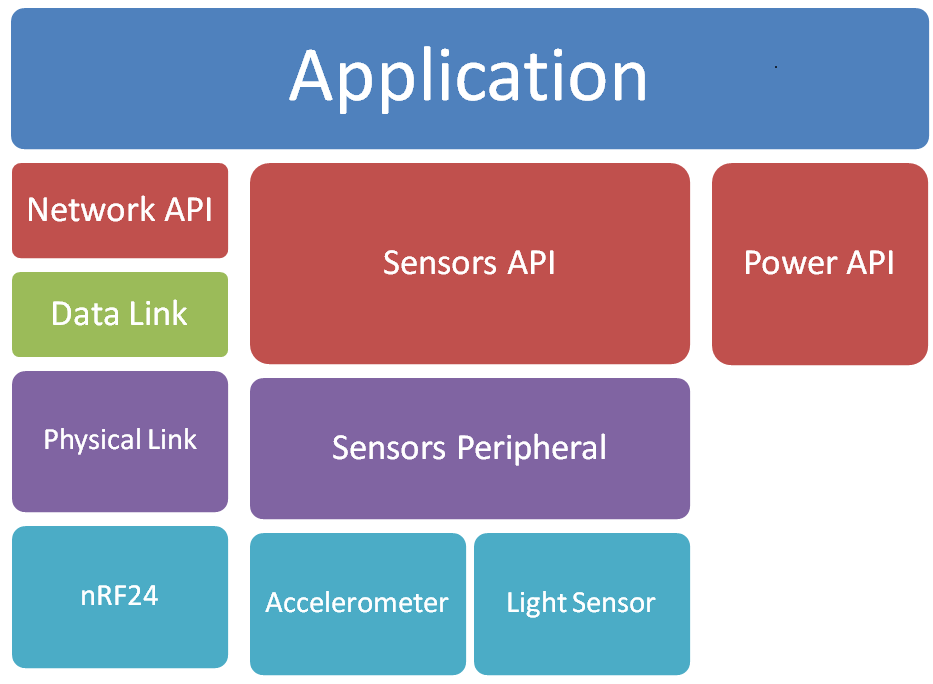
\includegraphics[width=0.5\textwidth, keepaspectratio=true]{images/archatechture.png}
  \end{center}
  \caption[System Architecture]{System Architecture}
  \vspace{-10pt}
\end{wrapfigure}

\subsection{Modularity}
Following the design of the modular system it was key to implement to system from the ground up
to support this reduced coupling. Each module is given and initialisation and de-initialisation call to
enable peripherals and data structures to be configured and also so after use all unnecessary
systems can be powered down. This de-initialisation was found to be most important during
development as the many of the peripherals continue to interact with the system after use, causing
faults.

Each module then has a public \ac{API} to simplify and abstract its internal processes. This is also
important as the C programming module does not support the protection of functions or variables
and so the use and separation of public interfaces allowed immediate warning throughout the use of
the compiler when functions or data where misused. The \ac{API} was used to abstract all data stored
locally in each module by the use of getters and setter forcing data localisation through the use of
coding conventions. These abstractions can be easily compiled out so does not incur a performance
reduction.

% TODO
\clearpage
\clearpage
\lstset{language=[ANSI]C, frame=single, caption={Module \ac{API}}}
\begin{lstlisting}
/* Called to (re)configure the module */
void init(void);
/* Called to configure the module only if not
 * already done so
 */
void required(void);
/* Called to asses the minimum sleep state the
 * system can achive */
sleep min_sleep(void);
/* Called to (re)configure the module if needed
 * after a sleep state */
void wakeup(sleep from);
/* Called to unconfigure the module */
void deinit(void);
\end{lstlisting}

% TODO DAVID PROOF %%%%%%%%%%%%%%%%%%%%%%%%%%%%%%%%%%%%%%%%%%%%%%%%%%%%%%%%%%%%%

The modularity of the code also assisted in reusability and supported the use of a readable single
code base. The entire system was hosted in a single code base, without the separation of node and
base station, and the use of a pre-processor was used to facilitate this. A pre-processor can lead to complex
and often hidden errors when used without modularity and so could be used more safely with the
modular system. Listing \ref{lst:PreProsError} show clearley that the pre-processor also aide the proggrammer
be producing compile time errors, saving the time required to flash the devices.

% TODO DAVID PROOF END %%%%%%%%%%%%%%%%%%%%%%%%%%%%%%%%%%%%%%%%%%%%%%%%%%%%%%%%%

\begin{minipage}[b]{0.5\linewidth}
  \vspace{+10pt}
  \begin{center}
    \lstset{language=[ANSI]C, frame=single, caption={Run-time Configuration}}
    \begin{lstlisting}
if (function == BASE) {
  run_base();
} else if (function == NODE){
  run_node();
} else {
  exit(EXIT_FAILURE);
}
    \end{lstlisting}
    %\caption[ToDo]{ToDo}
  \end{center}
\end{minipage}
\hspace{0.1cm}
\begin{minipage}[b]{0.5\linewidth}
  \vspace{+10pt}
  \begin{center}
    \lstset{language=[ANSI]C, frame=single, caption={Compile-time Configuration}, label=lst:PreProsError}
    \begin{lstlisting}
#if FUNCTION == BASE
  run_base();
#elif function == NODE
  run_node();
#else
#error "Invalid 'FUNCTION'"
#endif
    \end{lstlisting}
    %\caption[ToDo]{ToDo}
  \end{center}
\end{minipage}


%%
%% Copyright Guy Taylor 2012
%%
%%

\chapter{Implementation and Testing}

\section{Development Environment}
Unlike traditional desktop development where the development code, compiler
and debugger are present on the same system, in embedded development the
roles are split across three devices. These systems are also mostly unstandardised
and need proprietary devices or software to function. Achieving a stable and
effective development environment enables more agile development and
helps assist rather than inhibit the programmer.

\subsection{Integrated Development Environment (IDE)}
I initially used the free ARM MDK IDE because it was being used in a concurrent Respire Project. I
found MDK to be unsatisfactory for my needs and moved mid-project to the Eclipse IDE, which is
one of the leading IDEs in the embedded development field, and in many others. I chose it because it
is fast becoming the industry standard and is being used as the basis for official ARM MD5 IDE.
Eclipse is also both open source and fully supported on Linux, enabling use without cost for this
project.

\subsection{Compiler}
The ARM Compiler tool chain (previously known as ARM RealView Compilation) used during the
initial stages. . I transitioned to the GNU Compiler Collation (GCC) during development to both
prevent vendor lock-in and enable the use of Linux as the host development environment. GCC was
used in the final and most successful development setup, superseding the ARM compiler which only
works on Windows(r) and is not fully supported using the GDB backend. The GCC compiler supports
a much larger number of processor targets , is available free of charge and is supported on both
Windows(r) and Linux. GCC is also fully supported by GDB and Eclipse. Specifically, I used Mentor
Graphics’ Sourcery CodeBench Lite Edition (formally Sourcery G++), a branch of GCC dedicated to
migrating the optimisation skew away from the x86 instruction set to the ARM family.
The use of the compiler’s pre-processor was core to the ability to enable a clean single code base
and remove unneeded runtime calculations. Many of the configuration settings were programmed
via the pre-processor and so could allow the user to reconfigure the system without reviewing
complex data sheets.
{inset code snippet}


\subsection{Debugger}
To achieve the aims of reducing vendor lock-in and provide a better environment to program in, the
GNU Project Debugger (GDB) was chosen. The GDB platform is the reference implementation of a
separated front and back end debugging system and the Mentor Graphics branch of this project was
utilised to best interact with the chosen compiler.


The debugging backend is highly coupled with the debugging emulator hardware adaptor used in the
project. The Energy Micro development boards used have an embedded SEGGER J-Link debugger
and therefore a SEGGER J-Link EDU debugger was chosen for consistency when an additional
debugging device was needed. The J-Link platform was chosen as it is well supported by Energy
Micro, works with GDB on both Windows(r) and Linux and supports the needed features. The Open
On-Chip Debugger project was tested but found to be too immature in its SWD debugging support,
as it could not correctly debug the system.


For additional ease of use, I produced a GDB proxy to implement a SWO viewer and work around
issues as they arose. A Python TCP GDB proxy was produced as the project continued and new
features were needed, which included:-
\begin{itemize}
  \item Managing multiple GDB connections to a single backend. The system will cleanly terminate
        the current connection allowing the new connection to take over. This is important as it
        prevents the Eclipse debugger from freezing for minutes at a time.
  \item Viewing of the raw GDB communications. Important in diagnosing the location of
        problematic events within the long opaque chain of systems.
  \item Displaying SWO output when enabled, separating the different types of information (e.g.
        printf, interrupts and timings). For the project environment using GDB, the system was
        unable to read live SWO output due to the SEGGER GDB server not passing the values on.
\end{itemize}


Integrating the powerful Eclipse debugging tool into this system allowed live code changes to be
made on the device as well as a clean GUI, enabling single stepping, expressions, variables and
advanced break point functions to be managed.


At the hardware level, I produced a 20pin JTAG/SWO connector to the 9pin Respire header. This
allowed quick insertion and removal of connectors without damaging the fragile header pins, whilst
also regulating the 5Volts supply to the required 3.3Volts. A small circuit was also produced to
enable error-free monitoring of SPI communications.
{insert pic}


\subsection{Digital Logic Probe}
Throughout the project implementation, it was important to be able to view the communications,
states and timings of the devices pins. To achieve this, an Open Bench Logic Sniffer digital probe was
used as it allowed:
\begin{itemize}
  \item The high accuracy of timing required, down to 5 nanoseconds.
  \item Automated decoding of SPI communication when linked to the Logic Sniffer software.
  \item Automated frequency and duty cycle calculations with error calculations.
  \item Multiple trigger configurations so only the required data was collected, enabling higher
        sampling rates.
\end{itemize}

\subsection{Developmental Hardware}
Throughout development, I used two EFM32-SDK development boards produced by the processor
manufacturer (Energy Micro HA) and a specially-adapted Respire unit which had a replacement
connection between the LETIMER and the NRF24 radio (inseret pin x and y; produced by J. Mann at
my request). This equipment was sufficient to test a 3-node network.

\section{Firmware}

\subsection{Nested Vector Interrupt Controller}
The Nested Vector Interrupt Controller (NVIC) of the Cortex-M3 was used to allow the system to be
more predictable. Given the event-driven design of my implementation, there is a higher risk of
interrupt coincidence, increasing delays in time-critical sections of code. To combat this potential
issue, I gave each interrupt a priority to allow the advanced interrupt controller to reorder the
interrupts.

{code nippet of NVIC SetPriority}

In many interrupts, I also chose to release the interrupt lock early to prevent missed events. This was
carefully planned in each occurrence as misuse of the feature can cause an infinite interrupt loop.
This more complex system was chosen as it works in bursts suitable for TDMA, with multiple time-
critical sections condensed together.


{code snippet to show interrupt reset}


I also utilised the Cortex-M3s SysTick feature in combination with the interrupt system to enable a
power efficient delay function for delays over 2msec.
{code snippet}


\subsection{Events and Interrupts}
Throughout the code base, I made extensive use of Wait For Interrupt (WFI), Wait For Event (WFE)
and Set Event (SEV), which are allowable in the Cortex – M3. These instructions set extensions,
facilitate reducing the inefficient nature of polling for change. The common implementation of the
‘while-loop’ polling for a required change of state prevents the system from powering down. By
using the above instructions correctly, I aimed to power down the system without introducing
latency, by configuring the loops to exit after an interrupt where appropriate.
{insert graph}


In events where a software interrupt was required, I used the SEV instruction, SEVs are more
efficient than interrupts for this purpose as they do not have an Interrupt Service Routine (ISR)
connected to their behaviour.


{insert code snippet}


\subsection{Peripheral Reflex System (PRS)}
The PRS unique to the EFM32 enabled me to implement a novel system to reduce the duty cycle.
This requires synchronisation of Real Time Clocks (RTC) on all devices sharing a common frequency. I
configured the RTC and the Low Energy Timer (LETIMER) on each device using PRS such that an RTC
pulse initiates the following sequence of events in each device at the beginning of every TDMA cycle
(of length specified in the network design):-
\begin{enumerate}
  \item The NRF24 enable pin is briefly pulsed on all devices (preconfigured where Respires are in
        Receive mode and Base Stations are in Transmit mode)
  \item The NRF24 enable pin is toggled on in the Base Station (in Receive mode)
  \item The NRF24 enable pin on each Respire device is pulsed sequentially (in Transmit mode) as
        determined by its unique network address
  \item The NRF24 enable pin on the Base Station is toggled off.
\end{enumerate}


This recurrent sequence is illustrated in Figure ZZ. The EFM32 microcontroller remains in a low-
energy state throughout each sequence, except for interrupts from the LETIMER (configured to
trigger when the NRF24 enable pin switches off) or the radio (on receipt or transmission of packet)
within the network section of the code.


Insert diagram here


During implementation of this system I encountered difficulties when enabling the PRS to co-
ordinate the RTC and LETIMER triggers, which had both worked independently. After further
research and analysis, it was discovered that the RTC and LETIMER are required to have the same
periodicity for this PRS configuration. I chose to increase the RTC period (away from the most
efficient value) to match that required by the LETIMER, which resulted in an insignificant power
increase which was likely to be far outweighed by the power efficiency gains of the PRS. (numbers
required)

\subsection{Implementation of Firmware Modules}
The Firmware was implemented to the design of Figure X by incorporating the modules and systems
described below.

\subsubsection{Serial Peripheral Interface (SPI)}
An initial baud rate of 1MHz was chosen to coincide with the Energy Micro application notes. At
1MHz the SPI USART runs at 10\% of the NRF24’s maximum and 7\% of the EFM32’s maximum (using
the current clock speed). At this rate, a successful 32byte packet and 2 byte command upload to the
radio took 150msec. In an attempt to improve the performance and reduce the duty cycle of the
system, I investigated whether increasing the SPI baud rate alone would help because the period of
many of the system events in the highest power states is dependent on the speed of data that can
be transferred to and from the NRF24. However, it was found that increasing the baud rate to 7MHz
(the EFM32 maximum) made no improvement.

After analysis using the digital probe (ref fig z.) it was found that although the period taken for each
byte decreased, the period between byte transmission did not change. This suggested that the MCU
was unable to sustain transfer with only a single buffer (note that a race condition may occur
without correct flushing of the transmit buffer due to an incorrect Chip Select Pin state). A fix was
attempted by the use of the double hardware buffer but I was unsuccessful due to a hardware flaw
in the EFM32 (ref needed).


\subsubsection{DataLink Module}
This module initialises and configures the NRF24 radio, uploads and downloads the packet data from
the network modules to the radio and manages radio power and state.


Insert code snippet


Insert table


During development it was found that there were many issues related to the correct
communication, state control, and timing of the NRF24 radio. Throughout development, consistent
issues arose concerning the radio as it did not perform as suggested by the device documentation.
During discussions with the designer of the Respire, Janick Mann, several interpretations of the
NRF24 specification were considered. Several simple test applications were implemented using 4
separate NRF42 radios on 2 different EFM32 development boards. One such test configured the
radio to broadcast an unmodulated carrier signal, the manufacturer’s recommended testing method
(Ref Constant carrier wave output for testing) which required specialized radio spectrum analysers
to detect and analyse the signal. Initially the NRF24 hardware was found to behave as expected, but
when more complex interactions with the radio were tested (e.g. a ping-pong firmware application)
the receive-transmit functions became problematic and no reliable solution was found.
Furthermore, during this testing we discovered that high frequency changes exacerbated the issue
and unfortunately high frequency transitioning is required for TDMA. Both myself and Janick Mann
concluded that the most plausible cause of this problem was due to the NRF24 entering the
‘standby- II’ state. Within this state it is only possible to transition to a receive state through a
lengthy reset process or by transmitting a new packet (which is unacceptable for TDMA). Several
modifications of the firmware were produced attempting either to prevent the NRF24 entering the
‘standby- II’ state or to progress it out of this state through a reset procedure. No permanent
solution was found within the time constraints of this project.


\subsubsection{Network Modules}
An initial implementation of both MCU and the lower power PRS systems were produced but these
could not be adequately tested to the required levels because of the problems described above.


\subsubsection{Real Time Clock}
The EFM32 has a built in 24-bit Real Time Clock (RTC) connected to the Respire’s 32.768KHz external
clock and so it was decided to use this to ensure that the system kept good time. I configured the
system to provide a clock reference down to 30.518 μseconds (discussed in PRS). This
implementation will also track time over successive RTC overflow events every 1.52days and
minimises interrupts from low-power states.


\subsubsection{SysTick}
The SysTick feature of the Cortex-M3 enables a dedicated priority interrupt connected to the MCU
clock. By setting an appropriate prescaler to the SysTick, a predictable periodic interrupt is created.
This periodic ‘tick’ is aimed at supporting pre-emptive Real Time Operating Systems (RTOS) {ref to
masters on this} but for this project it was utilised to produce a more efficient delay function.


In low-power systems, any delay run on the MCU should be avoided, as it wastes power on ‘empty’
cycles. However during firmware development, this feature is highly desirable. To enable delays with
power efficiency in mind, the SysTick was used to allow 1msecond increments of the delay to be run
in a lower energy state.


{code snipett of “old function”}


By utilising the Energy Micro’s Energy Profiler, I discovered that the example SysTick function
provided by Energy Micro was negatively impacting on the duty cycle. By modifying this function to
enabling the SysTick only during delays, I produced an effective solution to overcome this issue
without having to sacrifice the lower power delay.
{code snippet }

\subsubsection{Debug}
I implemented a debug module on the device to assist in the development process. This included full
support for interacting with the digital probe to produce and test accurate timings and
communications. I also developed an extended version of the Energy Micro SWO code to add
support for printing to the console of the development PC, linked to the produced SWO viewer.
Code snippet

\subsubsection{Newlib Library}
New lib is a small standard C library designed for use in embedded MCUs. With the C language there
is a standard core library of functions that allow the programmer to maintain code portability. The
use of many of these functions however are application specific in MCUs (e.g. where should the
console go and how to query the device for the time?) and therefore need to be written for the
device used. Newlib is a collection of many optimised implementations for a large number of
platforms, however it did not have specific functions for the EFM32. I chose to implement a subset
of these functions to allow the use of advanced features such as dynamic memory (i.e. malloc). The
choice of Newlib was made as it already included a core set of features generic to all Coretx-M3
processors and was the library supported by the compiler.
{insert snippet of the heap code}


%%
%% Copyright Guy Taylor 2012
%%
%%
\chapter{Discussion}

\section{The Respire radio}
The \ac{NRF24} radio was chosen for the Respire due to its low power utilisation
and its reduced complexity compared with competitors. Unfortunately for my specific
requirements in implementing \ac{TDMA}, the latter advantage was found to hinder
development. As a result of its basic interface it proved difficult to diagnose
apparent problems with the radio through a lack of status information and the
inability to easily monitor any radio communications.


As a result of this unforeseen project issue, significantly more time was spent
troubleshooting during development, thus reducing the time available to produce
an analysis of the network design. In hindsight, implementation of a non \ac{TDMA}
network (mainly \ac{FDMA} as it is still suitable for larger networks) would
circumvent the requirement for a final resolution of the discussed \ac{TDMA}
issue (section x). This alternative network design using \ac{FDMA}, although less
efficient, would have allowed the project to progress into the analysis of power
and network efficiency, not achieved in this project. This data would have then
allowed a cost-benefit analysis of additional complexity caused by a larger network
implementation. This would have allowed a discussion into the feasibility of
further development of this approach in later Respire versions.


My original approach to the implementation of the project was based around my
previous work with a sister device with a similar aim. More specifically, a
wireless sensor network using the ProSpeckz IIK, containing a CC2420 IEEE 802.15.4
radio configuration resembling that found in the Respire. This experience however,
was not sufficient to address the challenges impeding the progress of this project,
leading me to assume that the source of the difficulty lay out-with my implementation.
Of course, it is dangerous to assume that one's implementation is not flawed, so
with this in mind, over the course of the project, I designed several strategies
to isolate any possible issues. Working to a design methodology which promotes
reusability, I have outlined some of the relevant strategies below so that they
might be used to inform future development:
\begin{description}
  \item[\ac{NRF24} -- \ac{MCU} Communication Monitoring] \hfill \\
    Utilising an Open Bench Logic Sniffer digital probe (section {4.1.4}) to
    monitor the shared pins between the \ac{MCU} and radio was used throughout the
    project to validate firmware. Vital to the correct working of the \ac{NRF24} is
    both the correct configuration of its registers and accurate timing (in both
    communications and signalling). To address issues that arose during the first
    half of the project an effective methodology to measure and analyse the probe's
    data was developed. It was found that continuous analysis of the probe traces
    is key to effective testing in this situation. This continuous testing allowed
    changes with adverse effects, which may even not yet be noticed, to be identified
    and rectified early.
    
    An additional hardware circuit (section x) was used in a strategy to originally
    test if the \ac{LETIMER} was causing unknown signalling problems when a state is
    forced by direct \ac{GPIO} control. A secondary pin's signal was merged and
    monitored confirming this was not causing the issue being tested. Further use
    of this on other multiuse pins showed however that the \ac{SPI} \ac{CS} pin
    produced glitches when manually controlled whilst routed to the \ac{SPI},
    this was then simply fixed. As this circuit allowed multiple devices to be
    probed accurately at the same time it was utilised at the end of the project
    to allow accurate timing of transmissions.
  
  \item[Serial Console Printing via \ac{SWO}] \hfill \\
    As \ac{TDMA} and the radio itself is highly sensitive to timing constraints
    it was found single-stepping or break-point debugging produces its own effects
    on the results. To enable good debugging whilst maintaining normal code flow
    the \ac{SWO} pin was utilised. This was further simplified by adapting Newlib
    to support the use of \ac{SWO} through printf. (section {4.1.3})
  
  \item[Modular Testing] \hfill \\
    To identify if ``Standby-II'' state within the \ac{NRF24} was causing the issue
    (ref) in radio communications, or any other, many strategies where devised.
    By utilising the modular system, many rapid prototypes of solutions could be
    produced including: transmit and receive only solutions, ping-pong transfers,
    shortened chip enable periods, and \ac{MCU} only radio control. The results
    of these test demonstrated that there was an issue with transitioning between
    receive and transmit states however several other tests demonstrated the source
    of the problem due to a ``Standby-II'' state where proven to be inconclusive.
  
  \item[Hardware Testing] \hfill \\
    Utilising specialised spectrum analysers in the Dept of Informatics at
    Edinburgh University, the \ac{NRF24} test radios where placed into unmodulated
    carrier signal mode, the manufacturer's recommended testing method
    (Ref Constant carrier wave output for testing). None were found to be defective,
    removing the probability of defective hardware. This testing is combined with
    multiple use of all hardware (2xdevelopment board and 4xradio) during normal
    development.
  
  \item[Radio ``Sniffing''] \hfill \\
    I attempted to monitor radio communications both through the use of an
    Ubertooth spectrum analyser  in the addition to production of a radio sniffer
    using an \ac{NRF24} linked to a FTDI \ac{MPSSE}. Neither of these attempts 
    was able to detect \ac{NRF24} radio signals under any conditions, this is most
    likely due to the operation outside the devices specifications combined with
    unusual \ac{PHY} radio layer. However this should be further looked at as the
    ability to monitor radio traffic ``in the air'' would vastly improve troubleshooting.
\end{description}

Unfortunately the \ac{NRF24} radio is a fixed component of the Respire and could
not be replaced for testing of alternative radios. Therefore in my opinion, in order
for \ac{TDMA} to be applied successfully to a Respire network these problems with
the \ac{NRF24} will have to be overcome. This has recently become a greater priority
for the Respire section of the Speckled Computing group at Edinburgh University
because they are reaching the limitations of the simpler type of wireless system
currently in use.  I hope that this document detailing the issues around \ac{TDMA}
with the \ac{NRF24} will be of use to further developing the Respire and other
\ac{NRF24} products.

External to Edinburgh University, the \ac{NRF24} radio is currently used principally for use in wireless
keyboards and mice, with a maximum of 6 devices in each network. The recent family of Logitech
Unifying\textregistered devices, which allows these devices to to communicate with a single \ac{USB}
dongle, is one of the \ac{NRF24}'s largest known implementation. Within this type of configuration, devices do not need
to transition between transmit and receive states often and do not require synchronisation. I am
aware of two articles reporting successful implementation of a TDMA-based wireless sensor network
using the \ac{NRF24} family of radios \cite{GossipingMAC, DecentralizedTDMA} in other devices, which suggest that it should be possible to
use it within the requirements of the Respire project. From the information included in these
publications, I could not identify any significant differences between their approach and mine to
programming the \ac{NRF24}, although in both papers the NRF24L01 was used where as the Respire
contains the NRF24L01+. The stated difference between these two generations of \ac{NRF24} is that the
Respire version includes several hardware-accelerated networking features. I tested my system with
these features both enabled and disabled without any improvement.

\section{The Respire MCU}
The EFM32 appears to be an excellent choice for the Respire which, although not fully utilised in this
project, enables substantial power and lower energy improvements over the previous generations of
hardware. The consistency of the EMF32's pin configurations throughout its family of chipsalso
allows the MCU in the Respire to be replaced without need for a redesigned circuit board. This was
an an active design choice, as it allows the future Respire to use the EFM32 Cortex-M4, soon-to-be-
released, again reducing energy needs whilst improving performance by use ofa hardware floating-
point unit. This design to enable future change of EFM32 has again been used to reduce the time to
market by both allowing the immediate use of the Cortex-M3 line, with knowledge of the later
compatibility, and by using a more powerful chip allowing over time with optimisations lower power
replacements. I would of wished this design desision had also extended towards the radio circuitry.

%\section{Power Reductions}
%By Utilising the low-powe 32Khz clock on the EFM32 my design tried aimed to provide minumin MCU
%interation during the radio prosses. ...
%About the code in the respire that reduces it power in general and aid development
%Accuracy of the packet transmission time estimates

\section{Wireless Medical Devices and their Standardisation}

\subsection{Wireless Medical Device Standards}
At current there is no single standard for wireless medical equipment with many current viable
solutions. With each solution developed by competing organisations there is little sign that this
situation will change within the scope of the Respire project. It is however important when choosing
or developing a solution to review and analyse the competition.

\subsection{Bluetooth Lower Power}
The Bluetooth Special Interest Group and its Bluetooth standard is one of the most prevalent
Personal Area Networks (PAN) technologies. The next generation of the Bluetooth specification
includes a new Bluetooth Low Energy (BLE) sub-specification, specifically designed to address the
needs of sensor networks. BLE markedly reduces the power requirements for Frequency-hopping
spread spectrum that is prevalent in the full Bluetooth specification. BLE however has only just
become available with the recent finalisation of the standard, but it would be the most likely
alternative solution for the Respire.


\subsection{IEEE 802.15.4}
IEEE 802.15.4 provides a specification on many areas of a full wireless network, ranging from the
physical layer to the data to be sent over it. The broad approach of this specification has led to the
ZigBee standard, producing smaller more manageable standards to each application, including
health care. A second approach of managing the IEEE 802.15.5 specification has been to overlay the
IPv6 specification to produce 6LowPan.


\subsection{ANT}
ANT is a fully proprietary radio and network implementation designed to simplify the production of
wireless health care devices. As a recent and closed system, few devices have been produced
utilising its technology.


\subsection{\acf{ISM} Bands}
With the finite usable frequency ranges available to all wireless radio devices, and those devices that
emit radio interference, there are restrictive licensing systems in place. Licensing systems are
independently run by each country or region, but from 1980 a movement began to identify a set of
frequency bands that could be used worldwide without a licence \cite{ISMGen}.
With the introduction of the unlicensed (but still heavily restricted) \ac{ISM} bands,
communication via modern wireless equipment became a
widely-available possibility. A key 2.4 GHz band became the most popular for consumer electronics
communications due to its high bandwidth, long range and ability to pass through internal walls. This
convergence of signals into a single small band, , has created a crowded environment which,
compounded by the use of microwave ovens and other interference devices, needs powerful and
creative communication algorithms to penetrate and be reliable. The NRF24 uses Gaussian
frequency-shift keying to optimise throughput but does little to avoid interference. However it has
been shown that a frequency-hopping system to reduce the susceptibility to interference can be
implemented on the NRF24. (ref)


%\section{Related Work}
%
%\subsection{Edinburgh University}
%Edinburgh University, under the leadership of J Mann, has also produced a separate implementation
%of a radio interface for the Respire. This implementation was designed with power efficiency as the
%only goal. To this end the system is designed such that the radio is only on, and only broadcasts
%when data needs to be sent. This system therefore produces the most efficient power solution that
%could be implemented on the device, ignoring optimisations of the design. The system also uses the
%hardware accelerated ShockBurst\textregistered and MultiCeiver\textregistered system designed by Nordic Semiconductors.
%With a brief of a fully managed network system suitable for hospital use, this design was decided not
%to be suitable.Also by the extended use of the NRF24.the design has underused the features of the
%EFM32. With the ability for asynchronously clocked serial transfer automated by and interrupts and
%managed by the DMA not been utilised a similar chip could have been used.
%
%\subsection{Alabama University}
%To do

\section{Future Work}
I an attempt to improve the systems lower use it was found that the SPI connection to the radio is
under utilised by the use of a single buffer. I attempted To fix this issue with the use of the double
buffer but was unsuccessful due to a hardware flaw in the EFM32 (ref needed), where if the double
buffer and single buffer are used in the same application it is not reflected in the status of the buffer
free register. The issue was not overcome by the prescribed fix as the initial issue absorbed the time
allocated for the feature and therefore would be a good candidate for improving the system's
energy use. A secondary, and preferred, final solution for longer transfers would be to enable the
DMA and fully enable the EFM32 to power down the entire length of the transfer. I decided that the
DMA solution was out with the time constraints afforded to this section of the project and therefore
would also be a key step in improving the system's energy usage.
As many people believe strongly in their privacy, especially when concerning their medical records, it
should be considered if cryptography should be implemented on the system. This feature should not
impose as big an effect on the energy efficiency as most devices as the EFM32 has hardware
accelerated encryption, however it does not include any acceleration for hashes.



%%
%% Copyright Guy Taylor 2012
%%
%%

\chapter{Conclusion}

Although this project did not produce a final complete networking solution for the Respire, it has
developed firmware and analysed important aspects of system design that future work can build
upon. In particular, it has identified the onboard \ac{NRF24} radio as a weak link in the system required
to effect this particular solution. The Respire network is an excellent concept for improving patient
management and care (and also conceivably as a future as a health/fitness aid) and \ac{TDMA} is a
preferred protocol for implementing this network. If one of the new generation of low-power radios
(\eg Bluetooth Low Energy) is a suitable replacement to the \ac{NRF24} as a Respire device
modification, then I am confident that the firmware, debugging protocols and hardware connections
I have developed during this project will greatly facilitate testing and implementation of these
devices in a Respire network.



%%%%%%%%
%% Any appendices should go here. The appendix files should look just like the
%% chapter files.
\appendix
%%
%% Copyright Guy Taylor 2012
%%
%%
\chapter{Code Analysis}

To generate Figure \ref{fig:git_work_time} I utilised the \url{http://www.GitHub.com} ``Impact'' graphic.
The values from this graphic where subsequently amended to take account of commit
\texttt{ee91d95da7ed2e4d4779b48c7487ad86d37a1fb1} and
\texttt{1701925f0a310ea00a195e64fc0379ab963e1cf3} as these they contained a unproportional
amount of code not produced by myself.


created gcc version
  ee91d95da7ed2e4d4779b48c7487ad86d37a1fb1
  07-01-2012

created the GDB proxy
  d9aaa51e7ff5d0ed034394ca24cd5bb5e0094761
  07-01-2012

created the debug module:
  c198234eb5e72eaa36718fe5923b2c190acd5d12
  09-01-2012

created the newlib module
  7ff54e992224314404a202c366fcea095687a163
  17-01-2012

created the radio module
  7ff54e992224314404a202c366fcea095687a163
  17-01-2012


\chapter{ToDo}

\section{ToDo}
\begin{itemize}
  \item makefile
  \item graph wireless time sync vs wired to show that the dirift is not bad
  \item JTAG 20pin to SWD adaptor
  \item http://ieeexplore.ieee.org/Xplore/login.jsp?url=http%3A%2F%2Fieeexplore.ieee.org%2Fiel5%2F5639116%2F5654845%2F05656550.pdf%3Farnumber%3D5656550&authDecision=-203
  \item https://github.com/kevinmehall/nRF24L01-buspirate
\end{itemize}

(If you're wondering what all this weirdness is, check out\\
\url{http://www.subterrane.com/loremipsum.shtml})

Morbi ultricies. Proin consequat. Praesent consequat nulla a mauris.
Vivamus tellus. 





%% Choose your favourite bibliography style here.
\bibliographystyle{apalike}

%% If you want the bibliography single-spaced (which is allowed), uncomment
%% the next line.
% \singlespace

%% Specify the bibliography file.
\bibliography{references}

%% ... that's all, folks!
\end{document}

